% Slot 1 of the ICAIF '26 tutorial: the problem, Bayes for volatility models (15 minutes).
% Uses the tutorial's bayesops theme unchanged; compile with LuaLaTeX (the theme needs it).
% In the Overleaf project: upload this file and figures/slot1/, then Menu > Main document > slot1.tex.
% The figures come from tutorial/notebooks/slot1_intro.py through tutorial/slides/slot1/export_figures.py; one of them,
% same-short-end.pdf, from Heston's variance-swap formula alone.
% Dashes are typed as Unicode (–): the theme's title fonts do not turn -- into a dash.
% Speaker notes are in \note{}; Beamer prints them only with \setbeameroption{show notes on second screen}.
% Numbers on the main slides are SPY market facts (study S8), measured costs (C8) and results that hold by
% construction; slide 7's detail cites quick checks on simulated data, labelled as such and detailed in the backup.
% Placeholders in angle brackets (\todo) are for the presenters to fill in.
\documentclass[aspectratio=169]{beamer}

\usepackage[cover]{bayesops}
\noautothankyouframe
\usepackage{booktabs}
\usepackage{array}
\newcolumntype{L}[1]{>{\raggedright\arraybackslash}p{#1}}  % a table column set ragged right
\usepackage{tikz}
\usetikzlibrary{arrows.meta, positioning}
\usepackage{unicode-math}
\setmathfont{Latin Modern Math}

% ─── Slot 1 helpers (what this deck adds to the theme) ────────────────────────
\providecommand\highlight[1]{\textcolor{neonlake}{#1}}
\definecolor{orchid}{HTML}{C2187A}  % the figures' second colour
\definecolor{lagoon}{HTML}{1A9C86}  % the figures' third colour
\setbeamercolor{structure}{fg=neonlake}
\setbeamertemplate{enumerate item}{\color{neonlake}\insertenumlabel.}
\addtobeamertemplate{block begin}{}{\raggedright}

% A headline number: \stat{value}{label}{caption}
\newcommand\stat[3]{%
  \tikz\node[fill=neonlake!8, rounded corners=2pt, inner sep=4pt, text width=\dimexpr\linewidth-8pt\relax,
             align=flush left]{%
    {\footnotesize\color{aviation!80}#2}\\[1pt]
    {\fontsize{15}{17}\selectfont\TitleFont\color{neonlake}#1}\\[1pt]
    {\footnotesize\color{aviation!70}#3}};%
}
% Blocks in the colour of a definition, a reassuring result or a warning
\newenvironment{defblock}[1]{\setblockcolor{aviation}\begin{block}{#1}}{\end{block}}
\newenvironment{goodblock}[1]{\setblockcolor{lagoon}\begin{block}{#1}}{\end{block}}
\newenvironment{warnblock}[1]{\setblockcolor{orchid}\begin{block}{#1}}{\end{block}}
% A figure on its own centred line
\newcommand\fig[2]{\par{\centering\includegraphics[width=#1\linewidth]{figures/slot1/#2}\par}}
\newcommand\source[1]{\par\vfill{\fontsize{6.5}{8}\selectfont\color{aviation!60}#1\par}}
\newcommand\todo[1]{\textcolor{orchid}{$\langle$#1$\rangle$}}  % for the presenters to fill in
% The reading order of a main slide: \key is the one short line everyone reads, under the title; \pairs is an optional
% strip under the figure, at most three \pair label–value pairs of a few words each; \bignum is a headline number with a
% label and a small note. \detail is small grey text, used only on backup frames.
\newcommand\key[1]{{\large\TitleFont\color{aviation}#1\par}\vspace{0.4em}}
\newcommand\pair[2]{{\scriptsize\color{aviation!55}\MakeUppercase{#1}}\\[1pt]{\small\color{aviation}#2}}
\newcommand\pairs[3]{\par\vspace{0.5em}{\color{aviation!15}\rule{\linewidth}{0.4pt}}\par\vspace{0.3em}%
  \begin{columns}[T,onlytextwidth]\column{0.32\textwidth}#1\column{0.32\textwidth}#2\column{0.32\textwidth}#3%
  \end{columns}}
\newcommand\bignum[3]{{\centering{\fontsize{20}{24}\selectfont\TitleFont\color{neonlake}#1}\\[4pt]
  {\small\color{aviation}#2}\\[1pt]{\footnotesize\color{aviation!60}#3}\par}}
\newcommand\detail[1]{\par\vspace{0.5em}{\footnotesize\color{aviation!60}#1\par}}

\title[Slot 1 · Bayes for Volatility Models]{The Problem: Bayes for Volatility Models}
\subtitle{Slot 1 · Amortized Bayesian Calibration of Volatility Models}
\author{Francesco Muia}
\venue{ICAIF '26 Tutorial}
\location{Milan, Italy}
\date{14–15 November 2026}

\begin{document}

\titleframe
\setcounter{framenumber}{0}
\useclassicframetitle

% ════════════════════════════════════════════════════════════════════════════
% How every main slide reads: the title and one short key line (\key) are what everyone reads; the figure is the
% evidence; the strip of facts under it (\pairs, at most three label–value pairs of a few words) is optional.
% Explanations go in the speaker notes, never in sentences on the slide. Style: plain statements, in logical order;
% each key line follows from the previous one.

% 0:00–1:30 · The problem, aligned with De Spiegeleer, Madan, Reyners and Schoutens (2018)

\begin{frame}{The Problem}
\key{The calibrated parameters are \highlight{uncertain}, and so are the prices computed from them.}
\vspace{0.4em}
{\centering
\begin{tikzpicture}[
    box/.style={draw=aviation!35, fill=aviation!4, rounded corners=3pt, align=center, font=\footnotesize,
                inner sep=4pt, text width=2.05cm, minimum height=1.5cm},
    arr/.style={-{Stealth[length=4pt]}, aviation!70, line width=0.6pt}]
  \node[box] (q) {\textbf{Option quotes}\\[1pt] {\scriptsize by strike and expiry}};
  \node[box, right=0.38cm of q] (c) {\textbf{Calibration}\\[1pt] {\scriptsize parameters that fit the quotes}};
  \node[box, right=0.38cm of c, fill=neonlake!12, draw=neonlake!60] (m) {\textbf{Calibrated model}};
  \node[box, right=0.38cm of m] (p) {\textbf{Products not quoted}\\[1pt] {\scriptsize forward starts, cliquets}};
  \node[box, right=0.38cm of p] (b) {\textbf{The book}\\[1pt] {\scriptsize valuations, hedges, reserves}};
  \foreach \a/\b in {q/c, c/m, m/p, p/b} \draw[arr] (\a) -- (\b);
  \node[font=\footnotesize\bfseries, text=neonlake, above=3pt of m] {every day, for many underlyings};
  \node[font=\footnotesize, text=orchid, below=2pt of c, align=center] {parameters known\\only approximately};
\end{tikzpicture}\par}
\pairs{\pair{Frequency}{daily, for many underlyings}}{\pair{Pricing}{Fourier integrals or Monte Carlo}}
      {\pair{Seven models, one smile}{similar fits, different exotic prices}}
\source{De Spiegeleer, Madan, Reyners and Schoutens (2018); Schoutens, Simons and Tistaert (2004).}
\note{Models are calibrated to option quotes every day, for many underlyings, and used to price products that are not
quoted (De Spiegeleer et al.\ 2018). Realistic models are expensive to price: Heston needs Fourier integrals, rough
Bergomi needs Monte Carlo. The quotes determine the parameters only up to their error, so the prices of unquoted
products are uncertain. Schoutens, Simons and Tistaert (2004) fitted seven models to one Eurostoxx 50 smile; all fitted
well, and their prices of barrier, lookback and cliquet options differed substantially. Banks report this uncertainty
today using consensus data and expert ranges.}
\end{frame}

% ════════════════════════════════════════════════════════════════════════════
% 1:30–6:30 · The ingredients, on Black–Scholes and one close of SPY

\begin{frame}{The Data}
\key{The data are 63 SPY option prices, each with an \highlight{error band}.}
\fig{0.82}{smiles.pdf}
\pairs{\pair{Date}{close of 21 October 2026}}{\pair{Grid}{7 maturities $\times$ 9 strikes}}
      {\pair{Error band}{± 0.3 vol points at the money}}
\note{The chain has 13,114 options. Each expiry's implied volatilities are smoothed and read at fixed points: 7
maturities from one week to one year, and 9 strikes. Real and simulated smiles are read on the same grid. The error band
is an assumption of the tutorial: ± 0.3 volatility points at the money and ± 1 point in the wings, wider than SPY's
bid–ask spreads.}
\end{frame}

\begin{frame}{The Likelihood}
\key{The \highlight{likelihood} measures how well each value of $\sigma$ reproduces the observed price.}
\fig{0.86}{one-price.pdf}
\pairs{\pair{Model and data}{Black–Scholes, one 1-month price}}{\pair{Best fit}{$\sigma$ = 12.84\% ± 0.30 points}}
      {\pair{Likelihood}{$p(y \mid \sigma) \propto e^{-\chi^2(\sigma)/2}$}}
\note{The model maps $\sigma$ to a price; the observed price is the at-the-money 1-month price. Here
$\chi^2(\sigma) = (y - P(\sigma))^2/\sigma_c^2$, the squared difference in units of the error band. The error band of the
price, divided by the option's vega, gives the band of $\sigma$: 0.30 points.}
\end{frame}

\begin{frame}{Prior and Posterior}
\key{The \highlight{posterior} combines the prior with the likelihood. The prior matters only where the data are weak.}
\fig{0.84}{prior-sweep.pdf}
\pairs{\pair{Least squares}{the mode under a flat prior}}{\pair{Penalty toward yesterday}{a normal prior}}
      {\pair{Fixed parameter}{a prior of zero width}}
\note{With a prior of ± 2 points, the posterior mean moves by 0.15 points. With ± 0.3 points, the width of the data's
band, it moves halfway to the prior (16.4\%). With ± 0.1 points the prior dominates (19.3\%). Least squares, penalties
and fixed parameters correspond to particular priors.}
\end{frame}

\begin{frame}{Pricing Under the Posterior}
\key{Pricing a product under each posterior draw gives the \highlight{distribution of its price}.}
\fig{0.84}{put-range.pdf}
\pairs{\pair{Product}{1-month put at $\delta = -2$}}{\pair{90\% point}{43\% above the mark; linearized, 37\%}}
      {\pair{Prudent valuation}{uses the 90\% point}}
\note{The put's price is convex in $\sigma$, so its distribution is skewed, and a linear approximation underestimates its
90\% point. For a sold position the reserve is the 90\% point minus the mark. Prudent valuation (Regulation (EU)
2016/101) asks for this point; banks currently obtain it from consensus data or expert ranges.}
\end{frame}

\begin{frame}{Checking the Model}
\key{A \highlight{posterior predictive check} compares simulated quotes with the observed ones. Black–Scholes fails it on
SPY.}
\fig{0.84}{predictive-check.pdf}
\pairs{\pair{The put}{9.5 standard deviations away}}{\pair{The smile}{not reproduced by one $\sigma$}}
      {\pair{Models used next}{Heston, rough Bergomi}}
\note{The simulated quotes are prices under each posterior draw plus the error band. The market price of the put is 9.5
standard deviations from the prediction, and a single $\sigma$ cannot produce a smile. The notebooks therefore use
Heston, priced by Fourier integrals, and rough Bergomi, priced by Monte Carlo.}
\end{frame}

% ════════════════════════════════════════════════════════════════════════════
% 6:30–8:30 · What the quotes do not determine

\begin{frame}{Beyond the Quotes}
\key{Some quantities are not determined by the quotes. Their uncertainty is \highlight{set by the prior}.}
\fig{0.8}{same-short-end.pdf}
\pairs{\pair{Example}{Heston, quotes up to six months}}{\pair{Variance swap at two years}{21.3\% to 25.3\% across fits}}
      {\pair{Fixing it instead}{gives too narrow a range}}
\source{The curves come from Heston's variance-swap formula. Quick checks on simulated data: backup.}
\note{In Heston, quotes up to six months fix the average variance up to six months, but not how it continues. Three
parameter sets match those quotes and give 2-year variance-swap levels from 21.3\% to 25.3\%. Common practice fixes such
quantities, which is a prior of zero width, or fits them without a prior. On simulated data the first gives ranges that
are too narrow and the second ranges that are too wide (quick checks, backup).}
\end{frame}

% ════════════════════════════════════════════════════════════════════════════
% 8:30–11:30 · The cost of exact posteriors, and amortized inference

\begin{frame}{The Cost of Exact Posteriors}
\key{An exact posterior requires about \highlight{10,000 model evaluations}. A book or a validation requires thousands of
posteriors.}
\vspace{1.4em}
\begin{columns}[T,onlytextwidth]
\column{0.32\textwidth}\bignum{4 CPU-min}{Heston}{Fourier pricing}
\column{0.32\textwidth}\bignum{$\ge$ 17 CPU-h}{rough Bergomi}{85 min by importance sampling}
\column{0.32\textwidth}\bignum{no formula}{return histories}{hidden variance path}
\end{columns}
\source{One posterior per smile on one 4-core machine (C8, verified). The chain's cost is a lower bound.}
\note{Heston: 20 ms per evaluation, about 4 CPU-minutes per posterior. Rough Bergomi: 5 CPU-seconds per evaluation, at
least 17 CPU-hours per posterior by Markov chain Monte Carlo, about 85 CPU-minutes by importance sampling. For return
histories the likelihood requires integrating over the unobserved variance path. One posterior is affordable; thousands
are not.}
\end{frame}

\begin{frame}{Amortized Inference}
\key{A network is trained once on simulated data. It then returns posteriors for new data \highlight{in seconds}.}
\vspace{0.8em}
{\centering
\begin{tikzpicture}[
    box/.style={draw=aviation!35, fill=aviation!4, rounded corners=3pt, align=center, font=\scriptsize,
                inner sep=3pt, text width=1.72cm, minimum height=1.1cm},
    arr/.style={-{Stealth[length=4pt]}, aviation!70, line width=0.6pt}]
  \node[box] (prior) {\textbf{Prior}\\ plausible parameters};
  \node[box, right=0.32cm of prior] (sim) {\textbf{Simulator}\\ quotes or returns};
  \node[box, right=0.32cm of sim] (bank) {\textbf{A bank}\\ of simulated pairs};
  \node[box, right=0.32cm of bank, fill=neonlake!12, draw=neonlake!60] (net) {\textbf{Train a network}\\ once};
  \node[box, right=0.32cm of net] (draws) {\textbf{Posterior draws}\\ in seconds};
  \node[box, right=0.32cm of draws] (checks) {\textbf{Checks}\\ coverage, reference, predictive};
  \node[box, above=0.3cm of net, fill=orchid!8, draw=orchid!50, minimum height=0.55cm] (today) {\textbf{New data}};
  \foreach \a/\b in {prior/sim, sim/bank, bank/net, net/draws, draws/checks} \draw[arr] (\a) -- (\b);
  \draw[arr] (today) -- (net);
\end{tikzpicture}\par}
\pairs{\pair{New data}{1,000 draws in 1.4–3.6 s}}{\pair{Coverage test, 2,000 smiles}{about 2 CPU-h, not 2,800}}
      {\pair{Valid}{within the range of the prior}}
\source{De Spiegeleer et al.\ 2018; Horvath et al.\ 2021; Cranmer et al.\ 2020; BayesFlow: Radev et al.\ 2022.}
\note{The network is trained on parameter–data pairs simulated from the prior, and returns posterior draws for new data
directly. This is the idea of learned pricers (De Spiegeleer et al.\ 2018; Horvath et al.\ 2021), applied to the
posterior. A coverage test on 2,000 simulated smiles takes about 2 CPU-hours after a training bank of about 370
CPU-hours, compared with about 2,800 CPU-hours by importance sampling. The network is accurate only within the range
covered by the prior, so each notebook checks it.}
\end{frame}

% ════════════════════════════════════════════════════════════════════════════
% 11:30–14:30 · The afternoon, summary and presenters

\begin{frame}{This Afternoon}
\key{The three notebooks follow the same \highlight{five steps}.}
\vspace{0.6em}
{\centering
\begin{tikzpicture}[stage/.style={draw=neonlake!60, fill=neonlake!10, rounded corners=3pt, font=\small\bfseries,
                    text=aviation, inner sep=5pt, minimum width=1.9cm},
                    arr/.style={-{Stealth[length=4pt]}, aviation!70, line width=0.6pt}]
  \node[stage] (a) {model};
  \node[stage, right=0.45cm of a] (b) {simulate};
  \node[stage, right=0.45cm of b] (c) {train};
  \node[stage, right=0.45cm of c] (d) {infer};
  \node[stage, right=0.45cm of d] (e) {check};
  \foreach \x/\y in {a/b, b/c, c/d, d/e} \draw[arr] (\x) -- (\y);
\end{tikzpicture}\par}
\vspace{0.8em}
\small
\begin{tabular}{@{}L{0.27\linewidth}L{0.27\linewidth}L{0.38\linewidth}@{}}
\toprule
\textbf{Notebook} & \textbf{Data} & \textbf{Feature} \\
\midrule
Heston options & 63 option prices & an exact posterior for comparison \\
Rough Bergomi options & 63 option prices & a Monte Carlo pricer \\
Return histories & up to 5 years of daily returns & a hidden variance path \\
\bottomrule
\end{tabular}
\pairs{\pair{Next talk}{Amortized Bayes}}{\pair{Then}{Architectures}}{\pair{Worked cases}{synthetic, with known parameters}}
\end{frame}

\begin{frame}{Summary}
\vspace{0.8em}
{\large\TitleFont\color{aviation}
\begin{enumerate}\setlength\itemsep{1.3em}
\item Calibrated parameters are uncertain, and the prices computed from them inherit this uncertainty.
\item The posterior describes this uncertainty. The prior matters where the quotes are not informative.
\item Amortized inference makes posteriors fast enough for daily use and for validation.
\end{enumerate}\par}
\vfill
{\small\color{aviation!70}Next: Amortized Bayes.\par}
\end{frame}

\begin{frame}{Presenters}
\small
\begin{columns}[T,onlytextwidth]
\column{0.24\textwidth}\textbf{Francesco Muia}\\ {\footnotesize\todo{affiliation}}\\[4pt]
{\footnotesize This introduction; rough Bergomi options}
\column{0.24\textwidth}\textbf{Alexander Fengler}\\ {\footnotesize\todo{affiliation}}\\[4pt]
{\footnotesize Amortized Bayes; rough Bergomi options}
\column{0.24\textwidth}\textbf{Stefan T. Radev}\\ {\footnotesize\todo{affiliation}}\\[4pt]
{\footnotesize Architectures; Heston options}
\column{0.24\textwidth}\textbf{Jerry Huang}\\ {\footnotesize\todo{affiliation}}\\[4pt]
{\footnotesize Architectures; Heston options}
\end{columns}
\vspace{1.5em}
{\footnotesize Return histories: \todo{presenter}.\par}
\note{Assignments as in the curriculum of 24 October; confirm them, and who presents the return histories, before the
run-through.}
\end{frame}

% ════════════════════════════════════════════════════════════════════════════
\appendix
\section{Backup}

\begin{frame}{Backup: SPY's Option Chain}
\begin{columns}[T,onlytextwidth]
\column{0.26\textwidth}
\stat{13,114}{options in the raw chain}{35 expirations}\\[3pt]
\stat{5,358}{quotes kept after cleaning}{32 expirations}
\column{0.71\textwidth}\small
\textbf{Cleaning removes}
\begin{itemize}\footnotesize
\item in-the-money options: the out-of-the-money one carries the same information;
\item unreliable quotes: no bid, a crossed market, a spread over half the mid;
\item outliers, and expirations with fewer than 8 quotes.
\end{itemize}
\textbf{Standardized moneyness} \quad $\delta = \ln(K/F) / (0.2\sqrt{T})$\\[1pt]
{\footnotesize the distance from the forward, in standard deviations of a 20\% volatility}
\end{columns}
\fig{0.62}{chain-reach.pdf}
\end{frame}

\begin{frame}{Backup: How a Grid Price Is Read}
\begin{columns}[c,onlytextwidth]
\column{0.44\textwidth}\small
\textbf{The points}: 7 maturities, 1 week to 1 year, $\times$ 9 strikes, $\delta = -2, \dots, 2$.\par\smallskip
\begin{enumerate}\footnotesize
\item \textbf{Smooth} each expiration's implied volatilities.
\item \textbf{Read} the expirations before and after the grid maturity, at the grid strike.
\item \textbf{Interpolate} between them in total variance $\sigma^2 T$.
\end{enumerate}
\footnotesize 35 points come from two expirations, 28 from one. Nothing is extrapolated: beyond $\delta = 2$ the calls run
out, and those left cost less than their tolerance.
\column{0.54\textwidth}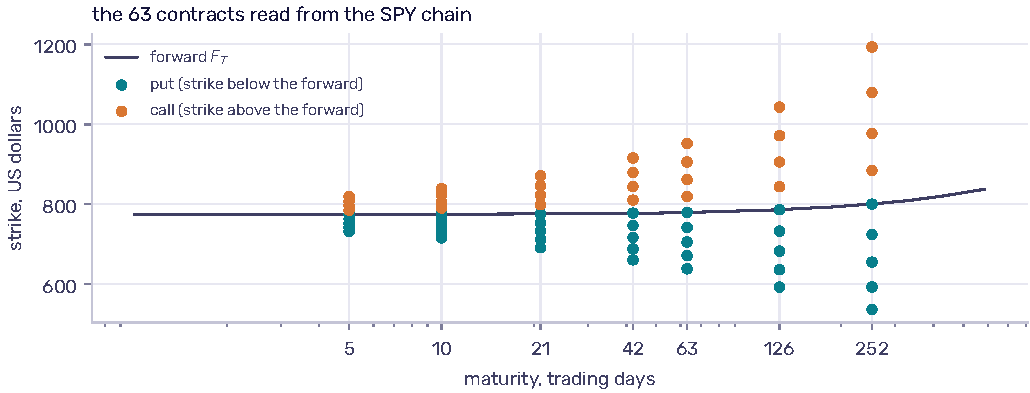
\includegraphics[width=\linewidth]{figures/slot1/grid-contracts.pdf}
\end{columns}
\end{frame}

\begin{frame}{Backup: The Tolerance of a Price}
\small Each grid price is the model's price plus an error of known size, set by a rule in two steps:
\[ \sigma_c = \underbrace{\mathrm{vega}_{20\%}(k_c, T_c)}_{\text{price per unit of volatility}} \times
  \underbrace{s(\delta_c)}_{\text{error in volatility}}, \qquad s(\delta) = 0.3 + 0.35\,|\delta| \text{ points.} \]
\fig{0.82}{noise-rule.pdf}
\begin{itemize}\footnotesize
\item \textbf{More than the quote}: the bid–ask, the grid reading and the model's own error. SPY's half-spreads sit
below the rule at every grid point.
\item \textbf{One rule for every smile}, real or simulated: a network trained on simulations then reads real quotes as
the same kind of data. At one month and the money, one volatility point is 11.5 bp of the forward, about \$0.89.
\end{itemize}
\end{frame}

\begin{frame}{Backup: What a Price Says About Volatility}
\fig{0.72}{quote-information.pdf}
\footnotesize
The error bars are the implied volatilities of each grid price $\pm$ its tolerance. At the money a 1-month price fixes
the volatility to $\pm 0.3$ points. At $\delta = 1.5$ and 2 the bars reach zero: those calls cost less than their
tolerance, so any lower volatility fits them. On 16 of 32 expirations the calls stop before $\delta = 2$; at one week
the $\delta = 2$ call costs \$0.01 against a tolerance of \$0.06.
\end{frame}

\begin{frame}{Backup: Level, Skew and Curvature}
\fig{0.9}{smile-shape.pdf}
\footnotesize The one-month smile with the parabola through the five quotes nearest the money; the level by maturity;
skew and curvature by maturity on log–log axes. The skew falls like $T^{-0.32}$.
\end{frame}

\begin{frame}{Backup: What a Network Reads}
\fig{0.9}{noise-units.pdf}
\footnotesize SPY's prices in units of their tolerance, $y_c / \sigma_c$: from 0.2 (one week, $\delta = 2$) to 56
(one year, at the money).
\end{frame}

\begin{frame}{Backup: The Variance Curve}
\fig{0.9}{variance-curve.pdf}
\footnotesize SPY's forward-variance levels and variance swaps, replicated from the option strip on 17 of 32
expirations: the curve rough Bergomi takes as an input, or infers.
\end{frame}

\begin{frame}{Backup: Assumptions Beyond the Quotes, in Practice}
\footnotesize
\begin{tabular}{@{}L{0.28\linewidth}L{0.13\linewidth}L{0.5\linewidth}@{}}
\toprule
\textbf{Not determined by the quotes} & \textbf{Common practice} & \textbf{Effect, on simulated data} \\
\midrule
A parameter: $\kappa$ (Heston), $\beta$ (SABR), $H$ (rough Bergomi) & Fix it & $H$ fixed at 0.10: the truth lies
above the 90\% bound on 23\% of thin chains, not 10\% \\
The variance curve beyond the last quote & Hold it flat & SPY's long end: 0.30–0.32 of the posterior's range for a
forward start and a 5-year put; zero for a 3-year variance swap \\
A name that barely quotes & Mark it from a proxy & 90\% intervals cover 59.5\%; with a hierarchical prior, 88.0\% \\
Any of these & Fit with no prior & Thin chains: 76 of 100 fits on a bound, ranges 1.5–3.3 times the posterior's.
Heston: no interval on 11 of 200 \\
\bottomrule
\end{tabular}
\detail{Each practice corresponds to a prior of zero width, or to no prior. Where the course measured it, a prior with
a stated width avoided both effects, and a Gaussian at the mode with the same prior did as well as the posterior. The curves of slide 7 come
from Heston's variance-swap formula, $\theta + (v_0 - \theta)(1 - e^{-\kappa T})/(\kappa T)$, with illustrative levels.}
\source{Quick checks on simulated data, not accepted studies (course, Lectures 8.10, 15.6, 16.4); Heston: study S6
(C11, verified). Practice: Hagan et al.\ 2002; Bergomi 2003; Janek et al.\ 2011; QuantLib, ORE; Reg.~(EU) 2016/101,
Art.~3(3)(a). Fixing $H$ is our analogy.}
\end{frame}

\begin{frame}{Backup: The Evidence in Detail}
\scriptsize
\begin{tabular}{@{}L{0.2\linewidth}L{0.75\linewidth}@{}}
\toprule
\textbf{Case} & \textbf{What was measured} \\
\midrule
Thin chains (quick check; course, Lecture 16.4) & 100 simulated chains with EWG's layout (27 quotes to six months), six
products, truths drawn from the prior. $H$ fixed at 0.10: truth above the upper bound on 23\% of chains for the variance
swap and the put (10\% nominal; about $\pm 6$ points at 95\%). Gauss–Newton with no prior: 76 fits on a bound, median
condition number $2 \times 10^{12}$, bands 1.5–3.3 times the posterior's, breached 0–7\%. A Laplace approximation with
the same prior: widths within 5\% of the posterior's. On 10 audited chains the network's bands are 1.04 times the exact
ones (median). \\
SPY's long end (quick check; Lecture 15.6) & Laplace posterior; beyond SPY's LEAPs the curve follows a random walk
with a standard deviation of 0.2 per square-root year. Flat extrapolation gives 0.32, 0.30 and 0 of the posterior's 90\%
range for a 2-to-3-year forward start, a 5-year put at 80\% and a 3-year variance swap. The forward start's range goes
from 19.4\% to 36.8\% of its price as that standard deviation goes from 0.1 to 0.3: the prior must be stated and tested. \\
A sector of names (quick check; Lecture 8.10) & 600 simulated Black–Scholes sectors of 2 liquid and 6 illiquid names.
Coverage of 90\% intervals: one name at a time 89.7\% (width 9.9 points), proxy 59.5\% (8.2), empirical Bayes 69.7\%
(5.5), hierarchical Bayes 88.0\% (7.6). Error of an unquoted 6-month call's mark: 10.2\%, 12.4\%, 8.5\%, 7.9\%. The
model is right by construction. \\
Heston, 200 smiles (study S6; C11, verified) & Gauss–Newton 90\% coverage 87–92\%, the network posterior's 87–90\%: on a
liquid, well-identified smile the classical route works. The optimum is on a bound of the box on 15 smiles; on 11 the
information matrix, computed in the search's logit coordinates, is singular and no interval exists. \\
\bottomrule
\end{tabular}
\end{frame}

\begin{frame}{Backup: Where the Posterior's Shape Matters}
\footnotesize
\begin{tabular}{@{}L{0.22\linewidth}L{0.73\linewidth}@{}}
\toprule
\textbf{Mechanism} & \textbf{Example} \\
\midrule
A price convex in a parameter & The put of slide 5: a sold put's reserve is 43\% of its mark
under the posterior, 37\% by the delta method. Exact. \\
A valley cut by bounds & Heston smiles with a fitted vol of vol below 0.3, 28 of study S6's 200: the skew pins only
$\rho\sigma_v$; Gauss–Newton's interval for $\sigma_v$ is 1.48 times the posterior's (median), and 6 smiles have two
or more optima. SPY sits far above, at $\sigma_v \approx 1.1$. Quick check (Lecture 11.6). \\
A bent ridge & Rough Bergomi with the curve inferred, one simulated smile: the posterior's 90\% range for the forward
variance from one to two years is 0.37 times Gauss–Newton's, skewed down; holding the curve flat puts it 21\% low and
the 2-year put 7.4\% low. Quick check (Lecture 15.6). \\
Two optima & Heston with jumps, synthetic surfaces: two optimizer end points with almost equal fit; a variance swap's
posterior range from $-18\%$ to $+67\%$ of its true price. Study of 9 October, not a registered claim. \\
\bottomrule
\end{tabular}
\end{frame}

\begin{frame}{Backup: Computing a Posterior}
\footnotesize
\begin{tabular}{@{}L{0.26\linewidth}L{0.32\linewidth}L{0.33\linewidth}@{}}
\toprule
\textbf{Method} & \textbf{Needs} & \textbf{Here} \\
\midrule
A grid & one or two parameters & Black–Scholes, in this talk \\
A Gaussian (Laplace) approximation & a posterior close to a normal, at one mode & thin chains, with the prior \\
Markov chain Monte Carlo & about $10^4$ evaluations of the model & Heston: minutes; rough Bergomi: $\ge$ 17 CPU-h \\
Importance sampling & a good proposal, such as a Gauss–Newton fit & rough Bergomi on SPY: $\approx$ 85 CPU-min \\
Amortized inference & one training run on simulations & seconds per data set; checkable at scale \\
\bottomrule
\end{tabular}
\end{frame}

\begin{frame}{Backup: References}
\scriptsize
\begin{itemize}
\item Bergomi, L. (2003). Dynamic aspects of smile models. Société Générale, slides.
\item Commission Delegated Regulation (EU) 2016/101 (prudent valuation), Articles 3 and 9 to 11.
\item Cranmer, K., Brehmer, J., Louppe, G. (2020). The frontier of simulation-based inference. \textit{PNAS} 117(48),
30055–30062.
\item De Spiegeleer, J., Madan, D. B., Reyners, S., Schoutens, W. (2018). Machine learning for quantitative finance:
fast derivative pricing, hedging and fitting. SSRN 3191050.
\item Demeterfi, K., Derman, E., Kamal, M., Zou, J. (1999). A guide to volatility and variance swaps. \textit{Journal of
Derivatives} 6(4), 9–32.
\item Hagan, P., Kumar, D., Lesniewski, A., Woodward, D. (2002). Managing smile risk. \textit{Wilmott Magazine}.
\item Hernandez, A. (2017). Model calibration with neural networks. \textit{Risk}, June 2017.
\item Horvath, B., Muguruza, A., Tomas, M. (2021). Deep learning volatility. \textit{Quantitative Finance} 21(1), 11–27.
\item Janek, A., Kluge, T., Weron, R., Wystup, U. (2011). FX smile in the Heston model. In \textit{Statistical Tools for
Finance and Insurance}, Springer.
\item Radev, S. T., Mertens, U. K., Voss, A., Ardizzone, L., Köthe, U. (2022). BayesFlow: learning complex stochastic
models with invertible neural networks. \textit{IEEE TNNLS} 33(4), 1452–1466.
\item S\&P Global Market Intelligence (2023). \textit{Totem Service}.
\item Schoutens, W., Simons, E., Tistaert, J. (2004). A perfect calibration! Now what? \textit{Wilmott Magazine}, March.
\end{itemize}
\end{frame}

\end{document}
